\section{Fibonacci chain}
\subsection{Dummy}
\begin{frame}{The Fibonacci chain}
\(
\<{7cm}{\textbf{Fibonacci numbers}}

A simple rule for generating numbers:
\begin{align*}
	F_0 &= 1 \\
	F_1 &= 1 \\
	F_2 &= F_1 + F_0 = 2 \\
	F_3 &= F_2 + F_1 = 3 \\
	F_4 &= F_3 + F_2 = 5 \\
	F_5 &= F_4 + F_3 = 8 \\
	&\vdots
\end{align*}
\[
	F_{l+2} = F_{l+1} + F_l
\]

\>

\<{7cm}{\textbf{Fibonacci words}}

Letters instead of numbers, same rule:
\begin{align*}
	C_0 &= \B \\
	C_1 &= \A \\
	C_2 &= C_1C_0 = \lett{AB} \\
	C_3 &= C_2 C_1 = \lett{ABA} \\
	C_4 &= C_3 C_2 = \lett{ABAAB} \\
	C_5 &= C_4 C_3 = \lett{ABAABABA} \\
	&\vdots
\end{align*}
\[
	C_{l+2} = C_{l+1}C_l
\]
\>
\)
\end{frame}

% counter has to be defined outside of the frame, otherwise a new counter is created at each iteration of only
\newcounter{slideno}
\begin{frame}{Fibonacci word from above}
(Infinite) Fibonacci word: \ca\cb\ca\ca\cb\ca\cb\ca\ca\cb\ca\ca\cb\dots

\ca{} $\leftrightarrow$ horizontal step, \cb{} $\leftrightarrow$ vertical step

\centering
\forloop{slideno}{1}{\value{slideno} < 14}{%
\only<\theslideno>{\includegraphics[width=.7\textwidth]{img/2_part1/CP_fibo_\theslideno}}%
}
\end{frame}

\begin{frame}{Quasiperiodicity of the Fibonacci word}
\(
\<{9cm}
\centering
\includegraphics[width=1.\textwidth]{img/2_part1/CP_fibo_cut}
\>
\<{6cm}
\begin{itemize}
	\item average slope = inverse of the golden ratio ($\tau \simeq 1.6$)
	\item bounded fluctuations
\end{itemize}
$\to$ similar environments everywhere

$\to$ quasiperiodicity [Duneau, Katz 85]
\>
\)
\end{frame}

\begin{frame}{Cut-and-project}
\(
\<{9cm}
\centering
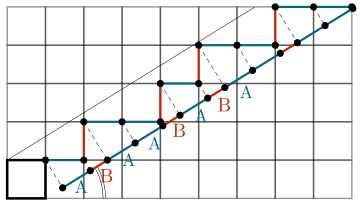
\includegraphics[width=1.\textwidth]{img/2_part1/full_cp}
\>
\<{6cm}
The cut-and-project algorithm:
\begin{enumerate}
	\item choose a hypercubic lattice (here $\zahl^2$)
	\item choose a ``physical plane'' $E_\parallel$ (here a slope)
	\item select points by translating the unit hypercube along $E_\parallel$
	\item project them onto $E_\parallel$.
\end{enumerate}
\>
\)

\textbf{\cp{} $\to$ quasiperiodic (or periodic) tiling!}
\end{frame}

\begin{frame}{From letters to atoms}
\begin{itemize}
	\item The Fibonacci word:
	\ca\cb\ca\ca\cb\ca\cb\ca\dots
	
	\item The Fibonacci (tight-binding) chain of atoms:
	
	{\centering
	%\documentclass[draft.tex]{subfiles}
%\documentclass{standalone}
%\usepackage{tikz}
%\begin{document}


    	\begin{tikzpicture}[scale=.6]
    		\newcommand{\orig}{-1.5}
    		\newcommand{\trans}{1.5}
    		\newcommand{\vertspac}{-2.}    		
    		\newcommand{\rad}{2pt} % radii of the circles
    		
    		% set the style of the strong bonds
    		\tikzset{
    			strong/.style={
    				double,
    				double distance=\rad,
    				line width=0.5pt
    				}
    		}
    	
    		% initial chain
    	
    		% bonds 
			\draw[-] (\orig+\trans,0) -- (\orig+2*\trans,0) node [midway, above] {$t_\ca$};
			\draw[strong] (\orig+2*\trans,0) -- (\orig+3*\trans,0) node [midway, above] {$t_\cb$};	
			\draw[-] (\orig+3*\trans,0) -- (\orig+4*\trans,0) node [midway, above] {$t_\ca$};
			\draw[-] (\orig+4*\trans,0) -- (\orig+5*\trans,0) node [midway, above] {$t_\ca$};
			\draw[strong] (\orig+5*\trans,0) -- (\orig+6*\trans,0) node [midway, above] {$t_\cb$};
			\draw[-] (\orig+6*\trans,0) -- (\orig+7*\trans,0) node [midway, above] {$t_\ca$};
			\draw[strong] (\orig+7*\trans,0) -- (\orig+8*\trans,0) node [midway, above] {$t_\cb$};
			\draw[-] (\orig+8*\trans,0) -- (\orig+9*\trans,0) node [midway, above] {$t_\ca$};
    	
    	
    		% sites
		    \filldraw (\orig+1*\trans,0) circle (\rad);% node [below] {6};
		    \filldraw (\orig+2*\trans,0) circle (\rad);% node [below] {3};
		    \filldraw (\orig+3*\trans,0) circle (\rad);% node [below] {8};
		    \filldraw (\orig+4*\trans,0) circle (\rad);% node [below] {5};
		    \filldraw (\orig+5*\trans,0) circle (\rad);% node [below] {2};
		    \filldraw (\orig+6*\trans,0) circle (\rad);% node [below] {7};
		    \filldraw (\orig+7*\trans,0) circle (\rad);% node [below] {4};
		    \filldraw (\orig+8*\trans,0) circle (\rad);% node [below] {1};
		    \filldraw (\orig+9*\trans,0) circle (\rad) node [right] {\dots};
		      
		\end{tikzpicture}

%\end{document}%
	}

\end{itemize}
Hamiltonian:
\[
	\op{H} = - \sum_m t_m \ket{m-1} \bra{m} + \hc
\]
Schrödinger equation for the eigenstate of energy $E$:
\[
	E \psi(m) = -t_{m}\psi(m-1) -t_{m+1}\psi(m+1)
\]
\end{frame}

\begin{frame}{A fractal state}
\centering
\includegraphics[width=.7\textwidth]{img/2_part1/heights_fibo}

\end{frame}